\titleformat % design des titres des chapitres
{\chapter}
[display]
{\centering\normalfont\Large\scshape\bfseries}
{\rule[3pt]{0.15\linewidth}{3pt}\quad\chaptertitlename~\thechapter\quad \rule[3pt] {0.15\linewidth}{3pt}}
{0\baselineskip}%espace vertical entre chapitre et nom du chapitre
{\rule{\linewidth}{0.5pt}\break\Huge}
[\vspace{-0.5\baselineskip}\rule{\linewidth}{0.5pt}\vspace{0\baselineskip}]

\let\clearpage\relax% Stop LaTeX from going to a new page; and
\vspace*{5.5cm}%

\chapter{Context general du projet}
Dans ce premier chapitre, je vais présenter l’entreprise d’accueil
DXC Technology Maroc à travers une description de l’historique ainsi
que son domaine d’activité et l’organigramme puis enfin une
présentation de ses clients.




\newpage
\section{Organisme d’accueil}
\subsection{Présentation de DXC Technology}

\begin{wrapfigure}{l}{0.42\textwidth}
  \begin{center}
    
\includegraphics[width=0.4\textwidth]{Rapport de stage PFE chez DXC/images/LogoDXC.png}
  \end{center}
\end{wrapfigure}
\\
HP-CDG IT Services Maroc est le fruit d’un partenariat stratégique
entre HPE (Hewlett Packard Enterprise), leader mondial du marché IT
et CDG (la Caisse de Dépôt et de Gestion)
\\
\\

Créée en 2007, HP-CDG IT Services Maroc a pu se positionner
rapidement parmi les acteurs leaders du conseil, des services informatiques et de
l’infogérance en profitant de l’expertise mondialement reconnu de HP. Ils développent
aujourd’hui une large gamme de conseils, de solutions et de services technologiques.
\\
\\
Précédemment connue sous le nom HP CDG IT Services Maroc, DXC Technology au Maroc est
née suite à un partenariat entre DXC Technology et la Caisse de Dépôt et de Gestion, cette nouvelle dénomination a pris effet le 3 Avril 2017 suite à la naissance de DXC Technology à travers une fusion entre Hewlett Packard Enterprise (HPE) et Computer Sciences corporation (CSC).
\\
\\
Cette fusion ayant donné naissance à l’un des plus gros acteurs de services aux entreprises au monde : DXC Technology, ce nouveau Groupe dispose d’un portefeuille de plus de 5900 clients répartis dans plus de 70 pays, dont le Maroc.
\\
\\
DXC Technology a été créée sur des fondations solides de confiance et de transformation et sur l’ambition renouvelée d’aider les clients à prospérer par le changement Digital. Ainsi, ils sont reconnus comme un multiplicateur de forces avec l’objectif principal d’apporter plus de valeur aux clients, aux partenaires et aux actionnaires de la société, et d’offrir davantage d’opportunités aux collaborateurs du groupe.
\\
\\
DXC Technology Maroc bénéficie de plus de 15 ans d’expérience dans le domaine informatique comptant plus de 1200 collaborateur qui travaille aujourd’hui en deux modes : hybride et distancielle.

\newpage
\subsection{Fiche signalétique de l’entreprise :}

Le tableau suivant présente la fiche signalétique de l’entreprise, c’est la carte d’identité de
l’entreprise.

\begin{figure}[h]
    \centering
    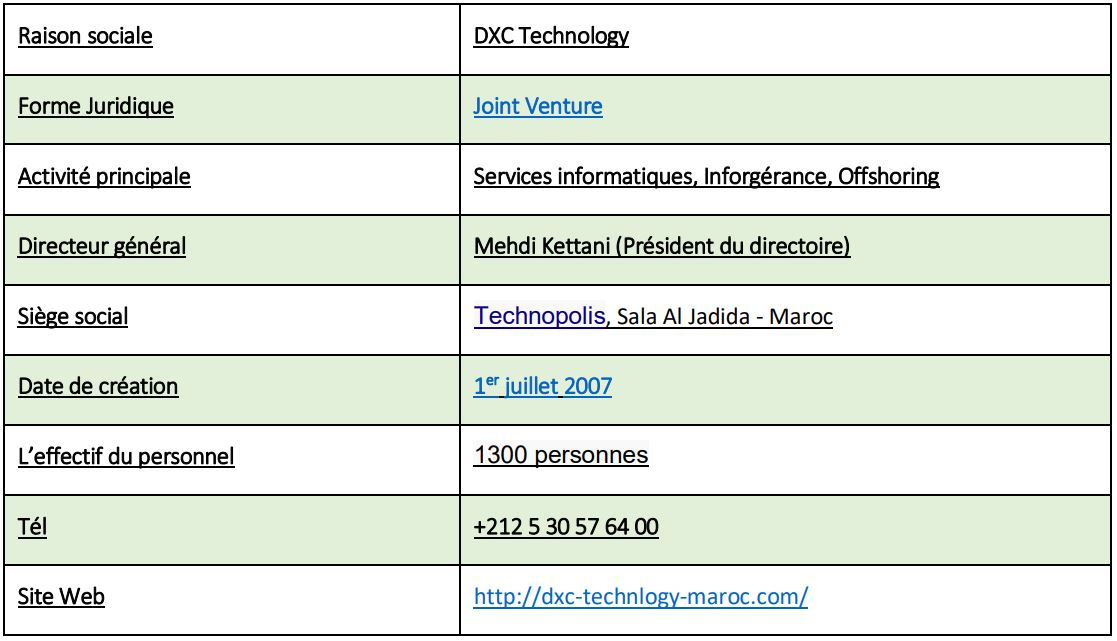
\includegraphics[width=\textwidth]{Rapport de stage PFE chez DXC/figures/fiche_entreprise.jpg}
    \caption{Fiche signalétique de l'entreprise}
\end{figure}

\newpage

\section{Historique et fait Marquants :}

La figure suivante présente l’évolution d’aventure de l’entreprise depuis 2007 jusqu’à 2014.

\begin{figure}[!h]
    \centering
    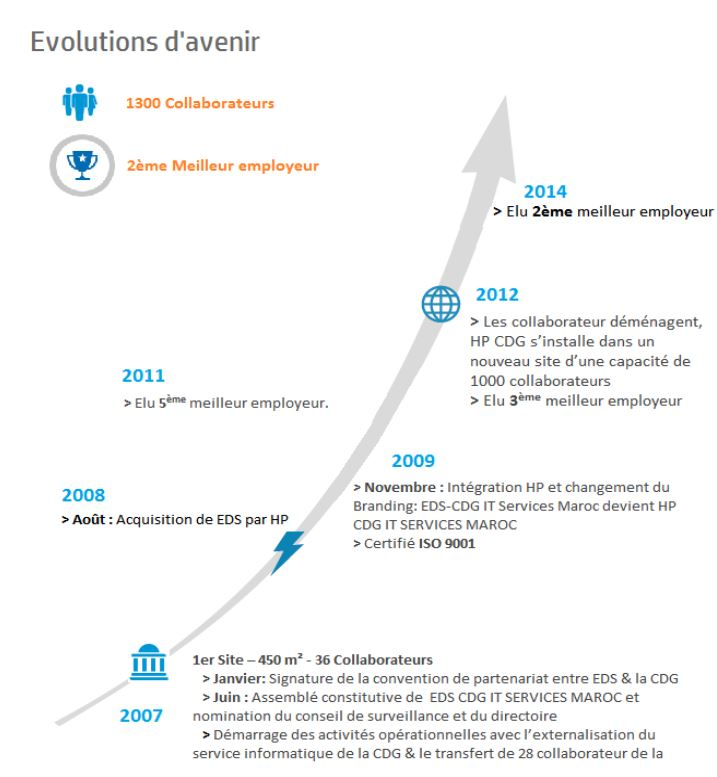
\includegraphics[scale=0.9,keepaspectratio]{Rapport de stage PFE chez DXC/figures/evolution_entreprise.jpg}
    \caption{Evolution de DXC Technology Maroc}
\end{figure}

\newpage
\subsection{DXC Technology histoire de succès :}

La figure suivante présente l’histoire de succès de l’entreprise DXC Technology et l’évolution du nombre des employés depuis 2007

\begin{figure}[!h]
    \centering
    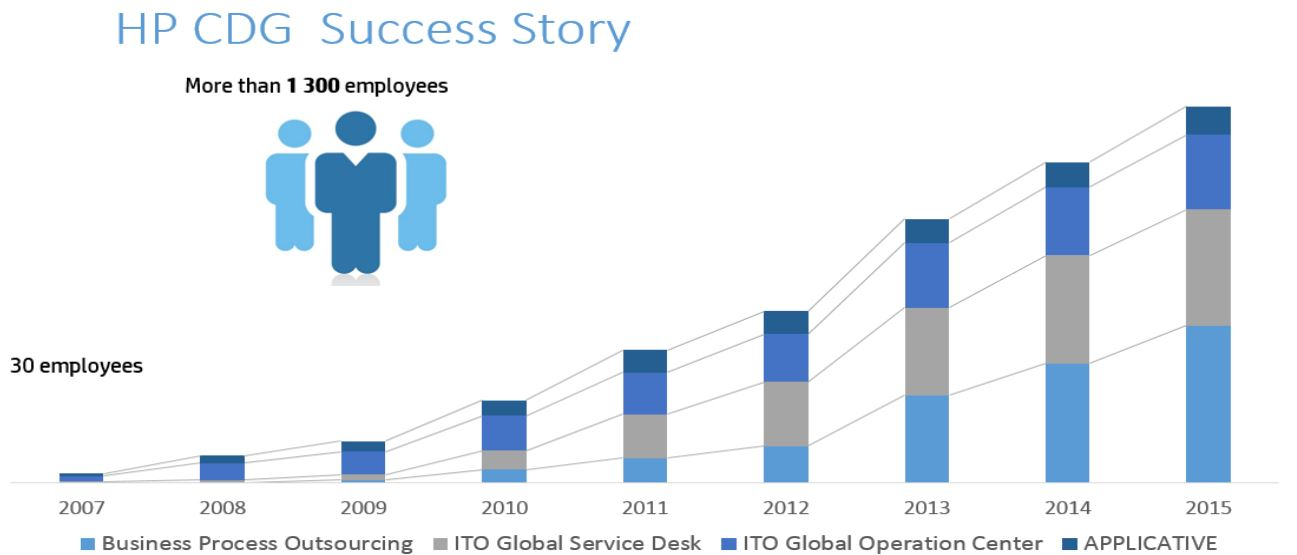
\includegraphics[scale=0.5,keepaspectratio]{Rapport de stage PFE chez DXC/figures/sucess_story.jpg}
    \caption{Histoire de succès de DXC Technology}
\end{figure}

\subsection{Secteurs d’activités:}

DXC Maroc délivre un large evantail de compétence :

\begin{figure}[!h]
    \centering
    \includegraphics[scale=0.4,keepaspectratio]{Rapport de stage PFE chez DXC/figures/compétence.jpg}
    \caption{Les clients de DXC Technologie Maroc}
\end{figure}

\newpage
DXC Technology est un centre de services qui dispose de ressources compétentes dans les
métiers de services informatiques suivants :

\begin{description}
  \item \textbf{Assurance:} La première mondiale des services et des solutions logicielles pour l’assurance. Soutient la croissance des assureurs, et amélien leur time-to-market et leur excellence opérationnelle grâce à des solutions d’assurance digitale et de gestion déléguée de leurs processus métiers.
  \item \textbf{Sante et Sciences de la vie:} Elle propose des logiciels leaders sur le marché et des services de gestion déléguée (BPS) pour les fournisseurs de soins, les payeurs, l’Etat et les entreprises de soins de santé. Elles se focalisent sur les soins cliniques et l’efficacité opérationnelle avec ses solutions de transformation digitale de soins.
  \item \textbf{Secteur public:} Ils sont un des leaders mondiaux de services informatiques indépendants et travaillent à tous les niveaux (Etat, administrations, collectivistes locales). Ils proposent pour les opérations et systèmes critiques une assistance 24 heures sur 24, et 7 jours sur 7.
  \item \textbf{Énergie:} Depuis plus de 20 ans, ils ont accompagné plus de 400 acteurs du secteur énergétique dans le monde entier. Leurs solutions les aident à saisir rapidement les opportunités du marché, se forger un avantage concurrentiel et mettre en œuvre de nouveaux modèles économiques.
  \item \textbf{Énergie:} Ils sont un desacteurs principaux des services informatiques dédiés aux secteurs Automobile, Équipements industriels, Chimie et High Tech. Ils allaient leurs solides connaissances sectorielles à des expertises spécifiques (Internet des objets, analytique, sécurité) pour aider leurs clients à doper leur innovation.
  \item \textbf{Communication, médias et divertissement:} Ils fournissent des solutions métiers innovantes aux acteurs du secteur Communication, médias et divertissement, aux quatre coins du monde, pour les aider à transformer leur organisation, réenchanter l’expérience client et tirer profit de la convergence digitale.
  \item \textbf{Aéronautique et défense:} Ils sont un des leaders des services informatiques dédiés au secteur Aéronautique et défense. Ils aident leurs clients à raccourcir leur time-to-market, prendre de meilleures décisions en exploitant la richesse de leurs données et adopter les technologies digitales. Ils accélèrent la mise en œuvre de l’innovation sur l’ensemble de la chaîne d’approvisionnement et de fabrication.
  \item \textbf{Transport et tourisme:} Avec plus de 40 ans d’expérience sur le marché, elle soutient les systèmes critiques du secteur (compagnies aériennes, passagers, fret, logistique, entreprises ferroviaires). Ses services aident leurs clients à soutenir leur croissance et les accompagne durant leur transformation.
  \item \textbf{Industrie:} Ils sont un desacteurs principaux des services informatiques dédiés aux secteurs Automobile, Équipements industriels, Chimie et High Tech. Ils allaient leurs solides connaissances sectorielles à des expertises spécifiques (Internet des objets, analytique, sécurité) pour aider leurs clients à doper leur innovation.
  \item \textbf{Distribution et grande consommation:} Ils aident les leaders mondiaux de la distribution et des biens de grande consommation se concentrer sur l’expérience client, et à saisir les opportunités liées aux nouvelles tendances digitales.
  \item \textbf{Communication, médias et divertissement:} Ils fournissent des solutions métiers innovantes aux acteurs du secteur Communication, médias et divertissement, aux quatre coins du monde, pour les aider à transformer leur organisation, réenchanter l’expérience client et tirer profit de la convergence digitale.
  \item \textbf{Aéronautique et défense:}Ils sont un des leaders des services informatiques dédiés au secteur Aéronautique et défense. Ils aident leurs clients à raccourcir leur time-to-market, prendre de meilleures décisions en exploitant la richesse de leurs données et adopter les technologies digitales. Ils accélèrent la mise en œuvre de l’innovation sur l’ensemble de la chaîne d’approvisionnement et de fabrication.
  
\end{description}

\subsection{Les clients de DXC Technologie Maroc :}

La figure suivante présente les différents clients et partenaires commerciaux de DXC.

\begin{figure}[!h]
    \centering
    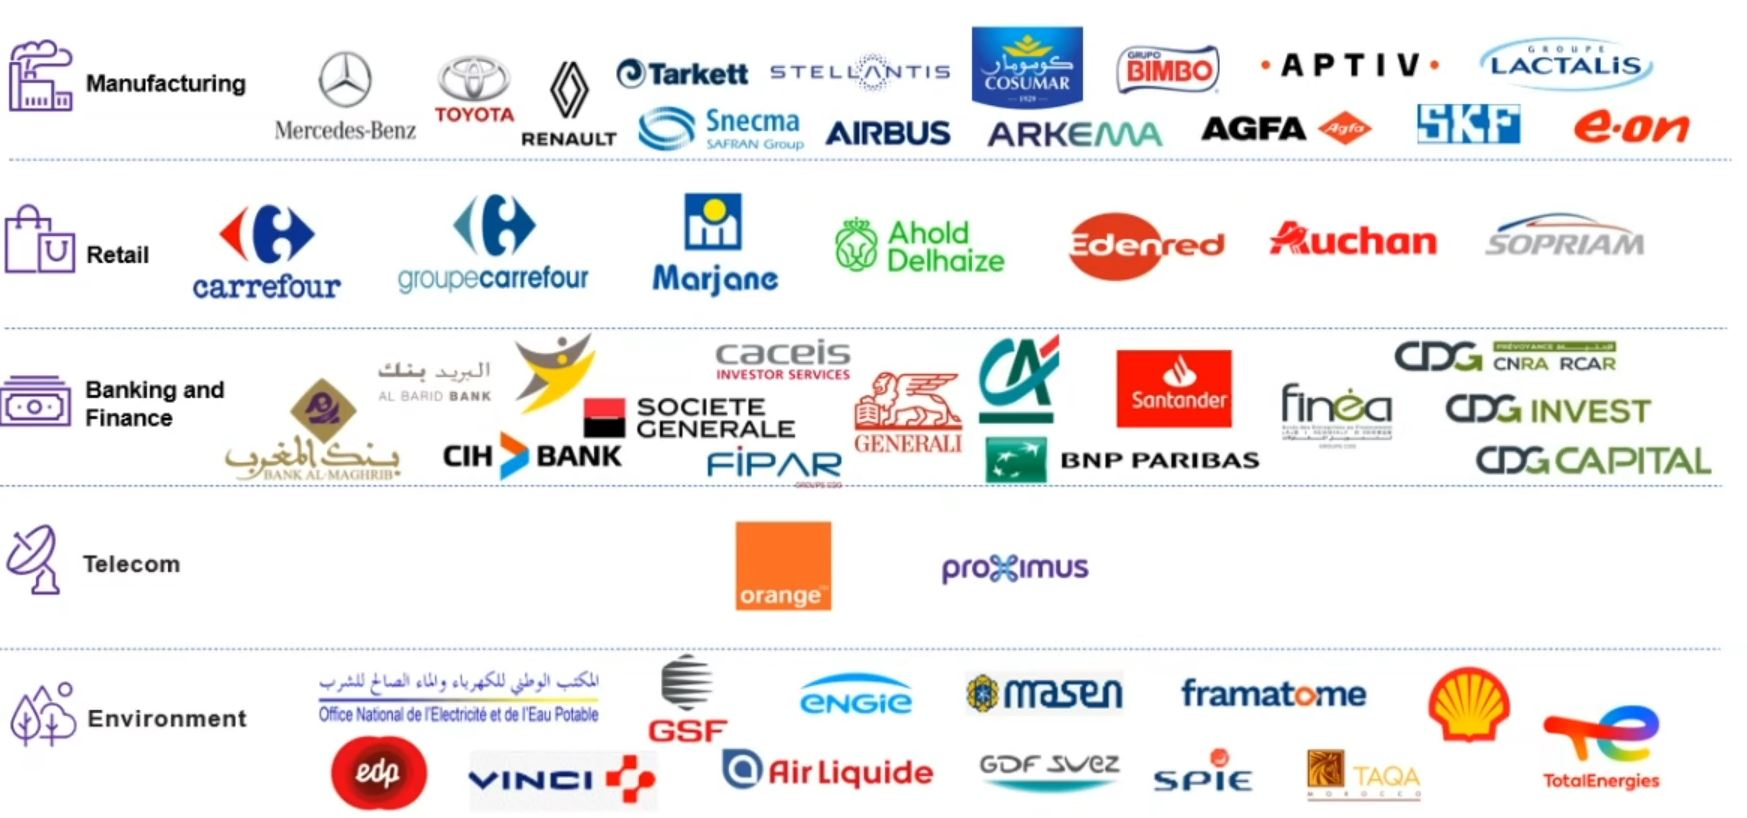
\includegraphics[scale=0.36,keepaspectratio]{Rapport de stage PFE chez DXC/figures/client.jpg}
    \caption{Les clients de DXC Technologie Maroc}
\end{figure}
\newpage
\subsection{Organigramme :}
La figure suivante présente quelques divisions principales de l’entreprise et pas la totalité
des divisions, il est divisé en 2 parties "Support" et "Services Lines" :

\begin{description}
  \item \textbf{Support :} rassemble l’ensemble d'activités de gestion considérées comme ne constituant pas le cœur de métier. Ces activités assurent le fonctionnement de l'entreprise et sont généralement communes à plusieurs divisions ou ligne de produits métier, tel que le service Finance, Ressources Humaines, marketing et service de ventes.
  \item \textbf{Service Lines :} contient les divisions qui représentent le cœur de métier, ces divisons
 sont :
 \begin{enumerate}
   \item \textbf{Application Services :} représente généralement les services de développement informatique et qualité logiciel, ainsi que l’intégration des ERP et le support applicatif.
   \item \textbf{Global Operations Services :} c’est une division dédiée pour les services d’Infrastructure, Cloud et Sécurité des systèmes d’information.
   \item \textbf{Business Process Outsourcing : } l’ensemble des activités qui ont comme but l'externalisation d'une partie de l'activité de l'entreprise vers un prestataire extérieur.
    \item \textbf{MWS  : } assure les services de gestion et support de mobilité, et le support au Delivery.
 \end{enumerate}
  
  \begin{figure}[!h]
    \centering
    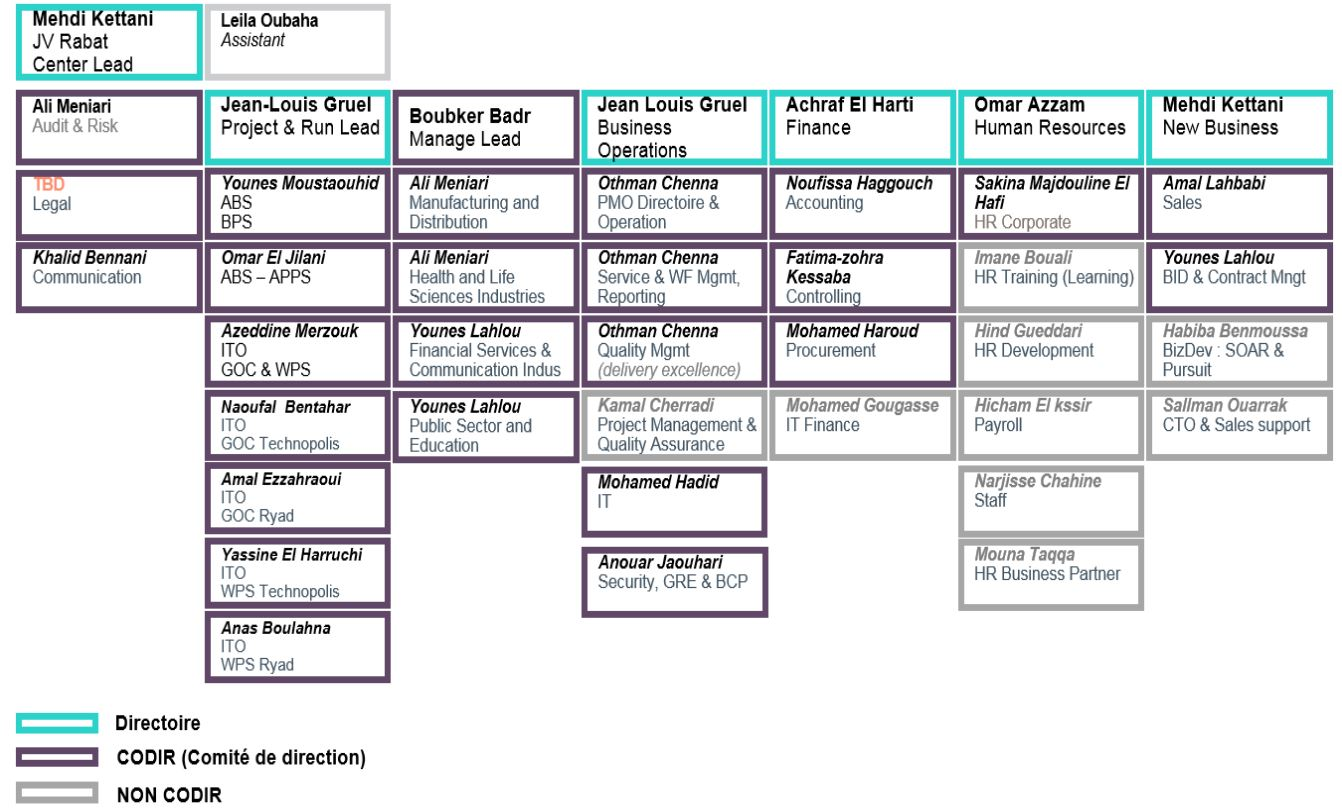
\includegraphics[scale=0.5,keepaspectratio]{Rapport de stage PFE chez DXC/figures/organigramme.jpg}
    \caption{Organigramme de DXC Technology}
\end{figure}
  
\end{description}


